\documentclass[conference]{IEEEtran}

\usepackage{amsmath,amssymb,amsfonts}
\usepackage{graphicx}
\usepackage{textcomp}
\usepackage{xcolor}
\usepackage{booktabs}
\usepackage{array}
\usepackage{listings}
\usepackage{url}
\usepackage{hyperref}
\usepackage{cite}

% Figurler ../figures/ klasorunde
\graphicspath{{../figures/}}

% Code Listing Style
\lstset{
	language=Python,
	basicstyle=\ttfamily\footnotesize,
	keywordstyle=\color{blue}\bfseries,
	commentstyle=\color{gray}\itshape,
	stringstyle=\color{red},
	numbers=left,
	numberstyle=\tiny\color{gray},
	numbersep=5pt,
	frame=single,
	breaklines=true,
	captionpos=b,
	tabsize=4
}

\def\BibTeX{{\rm B\kern-.05em{\sc i\kern-.025em b}\kern-.08em
		T\kern-.1667em\lower.7ex\hbox{E}\kern-.125emX}}

\begin{document}

	\title{Comparative Evaluation of Classification Algorithms for Bank Term-Deposit Subscription Prediction\\
		{\footnotesize BIL 476 / 573 --- Data Mining Course Project, Summer 2026\\
			TOBB University of Economics and Technology}
	}

	\author{\IEEEauthorblockN{Doruk Dolaşık}
		\IEEEauthorblockA{\textit{TOBB University of Economics and Technology}\\
			Ankara, Turkey \\
			Student ID: 211401030 \\
			ddolasik@etu.edu.tr}
	}

	\maketitle

	\begin{abstract}
		Direct marketing campaigns are costly, so banks benefit from predicting
		which clients are likely to subscribe to a term deposit before a call is
		made. This project addresses that classification problem using a public
		Bank Marketing dataset of 11,162 client contacts described by sixteen
		mixed-type attributes. Four supervised classifiers, namely Decision Tree,
		Gaussian Naive Bayes, k-Nearest Neighbors, and Random Forest, are compared
		under a unified preprocessing pipeline with standardized numeric features
		and one-hot encoded categorical features. Hyperparameters are selected with
		five-fold stratified cross-validation and models are evaluated on a held-out
		test set using accuracy, precision, recall, F1-score, and the area under
		the ROC curve. To assess the influence of a potentially leaking attribute,
		every model is trained twice: once with the last-contact call duration and
		once without it. Random Forest achieves the best performance in both
		settings, reaching an accuracy of 0.858 and an AUC of 0.921 with all
		features. Removing call duration lowers the best AUC to 0.786, confirming
		that this attribute carries information that is only available after the
		outcome is effectively decided. The study shows that ensemble methods offer
		a strong accuracy and robustness trade-off and that careful attribute
		auditing is essential for realistic performance estimates in marketing
		prediction.
	\end{abstract}

	\begin{IEEEkeywords}
		data mining, classification, random forest, bank marketing, data leakage
	\end{IEEEkeywords}

	\section{Introduction}
	\label{sec:introduction}

	Retail banks rely heavily on direct marketing, typically phone calls, to sell
	products such as long-term deposits. Because contacting every client is
	expensive and often intrusive, being able to predict in advance which clients
	are most likely to subscribe allows a bank to focus its effort, reduce cost,
	and improve customer experience. This makes term-deposit subscription a
	classic and practically valuable binary classification problem.

	The goal of this project is to answer two related questions. First, among
	several standard classification algorithms, which one predicts term-deposit
	subscription most accurately and reliably on a realistic client dataset?
	Second, how sensitive are these predictions to a single attribute, the
	duration of the last contact call, that is suspected of leaking outcome
	information? Answering the second question is important because a model that
	looks excellent on paper may be useless in practice if it depends on
	information that is not available at prediction time.

	To address these questions we use a public Bank Marketing dataset and compare
	four widely used classifiers: Decision Tree, Gaussian Naive Bayes,
	k-Nearest Neighbors, and Random Forest. All models share the same
	preprocessing and are tuned with cross-validation, so that differences in
	performance reflect the algorithms rather than the pipeline. Each model is
	trained in two scenarios, with and without the call-duration attribute, and
	compared with a consistent set of evaluation metrics.

	The remainder of this paper is organized as follows.
	Section~\ref{sec:related_work} reviews related work on the Bank Marketing
	dataset and on the classifiers used. Section~\ref{sec:dataset} describes the
	data and its characteristics. Section~\ref{sec:methodology} presents the
	preprocessing, algorithms, and experimental setup.
	Section~\ref{sec:results} reports the results, and
	Section~\ref{sec:discussion} discusses their meaning, limitations, and
	ethical implications. Section~\ref{sec:conclusion} concludes and outlines
	future work.

	\section{Related Work}
	\label{sec:related_work}

	The Bank Marketing dataset was introduced by Moro, Cortez, and
	Rita~\cite{b_moro}, who applied a data-driven approach to predict the success
	of bank telemarketing and reported that neural networks and support vector
	machines were competitive on the task. Their work also highlighted the strong
	predictive role of the call duration attribute, noting that it is only known
	after a call ends and therefore should be excluded when a realistic predictive
	model is required. Our study follows this observation directly by measuring how
	much performance depends on that single attribute.

	The classifiers we compare are well established in the data mining literature.
	Decision trees follow the recursive partitioning idea popularized by
	Quinlan~\cite{b_quinlan}, while Random Forest~\cite{b_breiman} improves on a
	single tree by averaging many de-correlated trees to reduce variance. The
	textbook by Han, Kamber, and Pei~\cite{b_han} provides the theoretical
	background for these methods as well as for Naive Bayes and k-Nearest
	Neighbors, including the interestingness and evaluation measures used in this
	work. Our implementation is built on the scikit-learn library described by
	Pedregosa et al.~\cite{b_sklearn}, which provides consistent implementations of
	all four algorithms and of the cross-validation and metric utilities we use.

	Compared with these studies, our contribution is not a new algorithm but a
	controlled, reproducible comparison on a single dataset that explicitly
	quantifies the effect of the leaking duration attribute across four classifiers
	under an identical pipeline.

	\section{Dataset Description}
	\label{sec:dataset}

	\subsection{Data Source}
	The dataset is the Bank Marketing dataset, originally collected from a
	Portuguese banking institution's direct marketing campaigns~\cite{b_moro} and
	distributed on Kaggle in a class-balanced form. Each record corresponds to one
	client contact, and the target variable \texttt{deposit} indicates whether the
	client subscribed to a term deposit. The dataset is appropriate for this
	project because it describes a real marketing decision, contains a mixture of
	numeric and categorical attributes, and is large enough for reliable
	model comparison.

	\subsection{Data Characteristics}
	Table~\ref{tab:dataset} summarizes the dataset. It contains 11,162 records and
	sixteen input attributes: seven numeric (age, balance, day, duration,
	campaign, pdays, previous) and nine categorical (job, marital, education,
	default, housing, loan, contact, month, poutcome). Unlike the original
	imbalanced version, this distribution is nearly balanced, which removes the
	need for resampling and lets us focus on algorithm behavior.

	\begin{table}[htbp]
		\caption{Dataset Summary}
		\begin{center}
			\begin{tabular}{|l|l|}
				\hline
				\textbf{Property} & \textbf{Value} \\
				\hline
				Number of Records & 11,162 \\
				\hline
				Number of Attributes & 16 (+ target) \\
				\hline
				Attribute Types & 7 Numeric, 9 Categorical \\
				\hline
				Target Variable & deposit (yes / no) \\
				\hline
				Missing Values (NaN) & 0 \\
				\hline
				Class Distribution & 52.6\% no / 47.4\% yes \\
				\hline
				Source & Bank Marketing (UCI / Kaggle) \\
				\hline
			\end{tabular}
			\label{tab:dataset}
		\end{center}
	\end{table}

	There are no explicit missing (NaN) values, but four categorical attributes
	use the token \texttt{unknown} as a placeholder: it appears in 70 job values,
	497 education values, 2{,}346 contact values, and 8{,}326 (74.6\%) of the
	\texttt{poutcome} values. The high proportion of unknown outcomes in
	\texttt{poutcome} reflects that most clients had not been part of a previous
	campaign, which is consistent with \texttt{pdays} being $-1$ (no prior contact)
	for the majority of records. Descriptive statistics for the numeric attributes
	are given in Table~\ref{tab:desc}. Balance is highly skewed, ranging from
	$-6{,}847$ to $81{,}204$ with a median of only $550$, and duration ranges from
	2 to 3{,}881 seconds.

	\begin{table}[htbp]
		\caption{Descriptive Statistics of Numeric Attributes}
		\begin{center}
			\footnotesize
			\begin{tabular}{|l|r|r|r|r|}
				\hline
				\textbf{Attribute} & \textbf{Mean} & \textbf{Std} & \textbf{Min} & \textbf{Max} \\
				\hline
				age & 41.23 & 11.91 & 18 & 95 \\ \hline
				balance & 1528.54 & 3225.41 & -6847 & 81204 \\ \hline
				day & 15.66 & 8.42 & 1 & 31 \\ \hline
				duration & 371.99 & 347.13 & 2 & 3881 \\ \hline
				campaign & 2.51 & 2.72 & 1 & 63 \\ \hline
				pdays & 51.33 & 108.76 & -1 & 854 \\ \hline
				previous & 0.83 & 2.29 & 0 & 58 \\ \hline
			\end{tabular}
			\label{tab:desc}
		\end{center}
	\end{table}

	Fig.~\ref{fig:class} shows the balanced target distribution, and
	Fig.~\ref{fig:cat} shows how the subscription rate varies across selected
	categorical attributes. Clients contacted with a successful previous outcome
	(\texttt{poutcome=success}) and those without a housing loan subscribe far more
	often than average, which already hints at informative structure in the data.

	\begin{figure}[htbp]
		\centerline{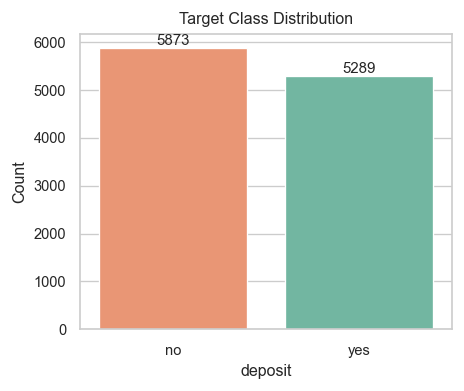
\includegraphics[width=0.72\linewidth]{class_distribution.png}}
		\caption{Target class distribution. The two classes are nearly balanced
			(52.6\% no, 47.4\% yes), so accuracy is a meaningful metric here.}
		\label{fig:class}
	\end{figure}

	\begin{figure}[htbp]
		\centerline{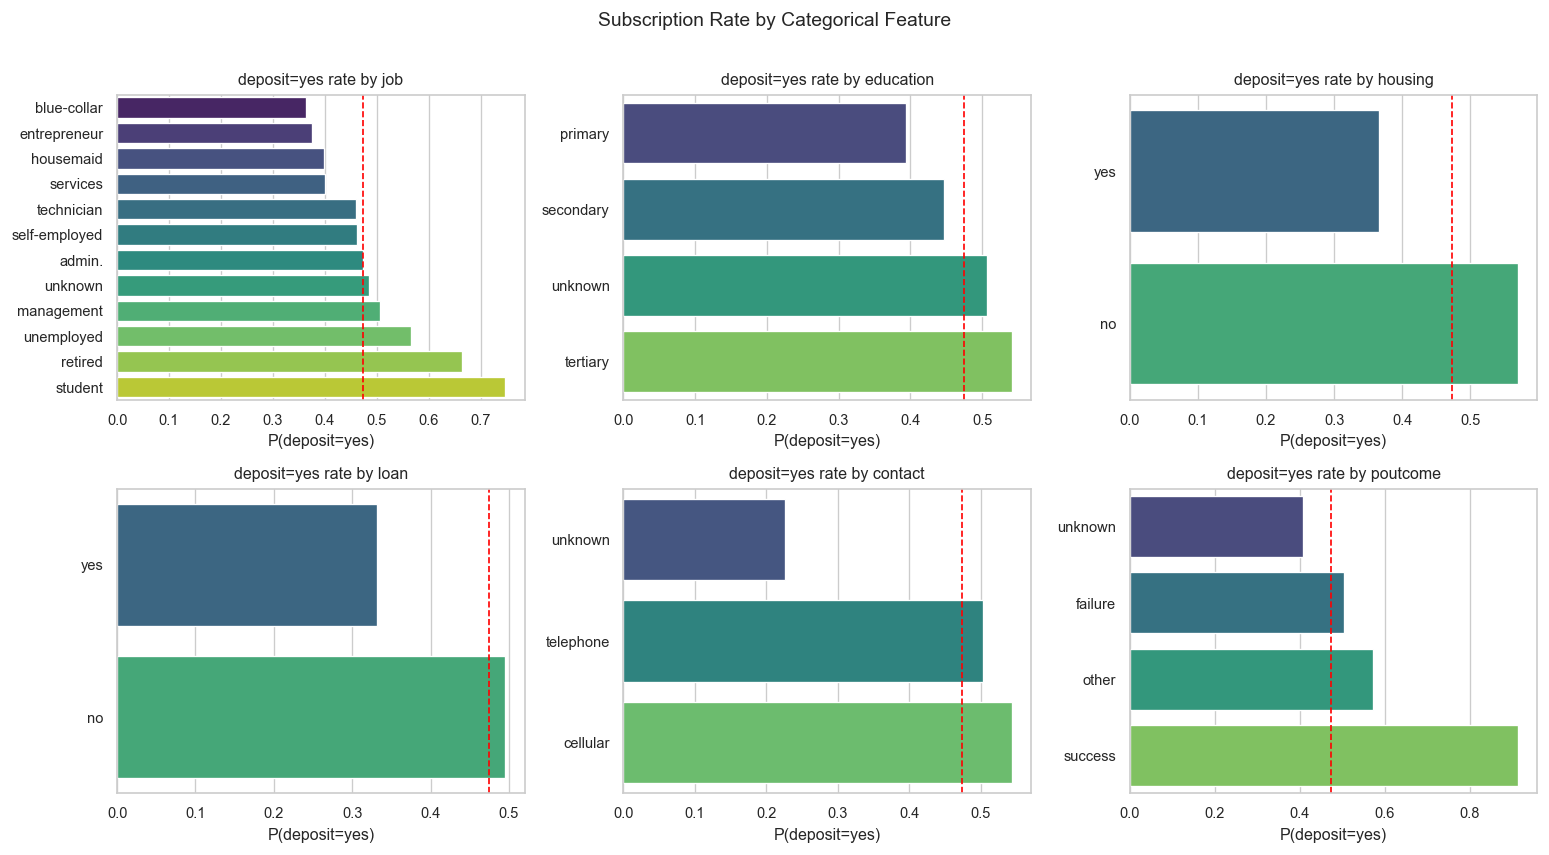
\includegraphics[width=\linewidth]{categorical_vs_target.png}}
		\caption{Subscription rate (deposit=yes) by categorical attribute. The red
			dashed line marks the overall positive rate. Previous-campaign success
			and absence of a housing loan strongly increase the subscription rate.}
		\label{fig:cat}
	\end{figure}

	\subsection{Ethical Considerations}
	The dataset contains no direct personal identifiers such as names or account
	numbers, which limits privacy risk. Nevertheless, attributes such as job,
	marital status, education, and age are socially sensitive, and a model that
	targets or excludes clients based on them could produce unfair treatment. Any
	deployed model should therefore be audited for demographic bias before use. No
	confidential or private data was uploaded to external AI tools during this
	project; only the public dataset and non-sensitive code were involved.

	\section{Methodology}
	\label{sec:methodology}

	\subsection{Data Preprocessing}
	A single preprocessing pipeline is shared by all models so that comparisons are
	fair. The steps are:
	\begin{itemize}
		\item \textbf{Target encoding:} the \texttt{deposit} label is mapped to
		1 (yes) and 0 (no).
		\item \textbf{Numeric scaling:} numeric attributes are standardized with
		z-score normalization. This is essential for the distance-based k-NN and
		beneficial for Naive Bayes, and it does not harm the tree-based models.
		\item \textbf{Categorical encoding:} categorical attributes are one-hot
		encoded, with unseen categories handled safely at test time. The
		\texttt{unknown} token is treated as its own category rather than being
		imputed, because for attributes such as \texttt{poutcome} the value
		``unknown'' is itself informative (no prior campaign).
		\item \textbf{No missing-value imputation} is needed, since the data
		contains no NaN values.
	\end{itemize}
	Preprocessing is fit only on the training split and then applied to the test
	split, preventing information leakage from the test data.

	\subsection{Algorithm Selection and Description}
	Four classifiers spanning different learning paradigms are compared:
	\begin{itemize}
		\item \textbf{Decision Tree} --- an interpretable model that recursively
		splits the feature space; used as an understandable baseline.
		\item \textbf{Gaussian Naive Bayes} --- a probabilistic model assuming
		conditional feature independence; fast and a useful contrast to the others.
		\item \textbf{k-Nearest Neighbors} --- a non-parametric, distance-based
		method that makes no assumption about the decision boundary shape.
		\item \textbf{Random Forest} --- an ensemble of decision trees that reduces
		variance through bagging and feature randomness, expected to be the
		strongest of the four~\cite{b_breiman}.
	\end{itemize}
	This selection satisfies the requirement of comparing multiple distinct
	approaches, covering interpretable, probabilistic, instance-based, and ensemble
	families.

	To study the effect of the leaking attribute, each classifier is trained under
	two scenarios: \emph{full} (all sixteen attributes) and \emph{no\_duration}
	(the same attributes minus call duration). This constitutes a second axis of
	comparison in addition to the four algorithms.

	\subsection{Experimental Setup}
	\begin{itemize}
		\item \textbf{Split:} an 80/20 stratified train/test split preserves the
		class ratio.
		\item \textbf{Model selection:} hyperparameters are chosen by five-fold
		stratified cross-validation on the training set, optimizing ROC-AUC via
		grid search. Tuned parameters include tree depth and minimum leaf size for
		the Decision Tree, the number of neighbors and weighting for k-NN, the
		number of trees and depth for Random Forest, and variance smoothing for
		Naive Bayes.
		\item \textbf{Environment:} Python 3.10 with scikit-learn 1.7.2, pandas,
		numpy, matplotlib, and seaborn.
		\item \textbf{Reproducibility:} a fixed random seed (42) is used for the
		split, cross-validation, and all stochastic models.
	\end{itemize}

	\subsection{Reproducibility and Verification}
	The full pipeline is deterministic given the fixed seed. The repository
	(Appendix~\ref{app:code}) contains \texttt{config.py}, \texttt{eda.py}, and
	\texttt{experiments.py}; running \texttt{experiments.py} regenerates every
	table and figure in this report. All numeric results reported here were
	produced directly by this code and independently inspected by the author.

	\section{Results}
	\label{sec:results}

	\subsection{Evaluation Metrics}
	Because the classes are balanced, accuracy is meaningful, but we also report
	precision, recall, and F1-score to capture the trade-off between missing
	interested clients (false negatives) and wasting calls on uninterested ones
	(false positives). The area under the ROC curve (ROC-AUC) summarizes ranking
	quality independently of the decision threshold and is used as the primary
	model-selection criterion.

	\subsection{Results Summary}
	Table~\ref{tab:full} reports test-set performance when all attributes are used.
	Random Forest is the best model on every metric except precision, achieving
	0.858 accuracy, 0.855 F1, and 0.921 AUC. k-NN is a strong second, while
	Gaussian Naive Bayes trails the others, largely because its independence
	assumption is violated by the correlated, one-hot encoded features.

	\begin{table}[htbp]
		\caption{Test Performance with All Features (full scenario)}
		\begin{center}
			\begin{tabular}{|l|c|c|c|c|c|}
				\hline
				\textbf{Model} & \textbf{Acc} & \textbf{Prec} & \textbf{Rec} & \textbf{F1} & \textbf{AUC} \\
				\hline
				Decision Tree & 0.808 & 0.767 & 0.855 & 0.809 & 0.891 \\ \hline
				Naive Bayes & 0.720 & 0.784 & 0.565 & 0.657 & 0.804 \\ \hline
				k-NN & 0.817 & 0.829 & 0.772 & 0.800 & 0.899 \\ \hline
				\textbf{Random Forest} & \textbf{0.858} & 0.825 & \textbf{0.888} & \textbf{0.855} & \textbf{0.921} \\ \hline
			\end{tabular}
			\label{tab:full}
		\end{center}
	\end{table}

	Table~\ref{tab:nodur} reports the same experiment with call duration removed.
	Every model degrades substantially: Random Forest's AUC falls from 0.921 to
	0.786 and its F1 from 0.855 to 0.673. The ranking of the models is largely
	preserved, with Random Forest still best, but the absolute performance is much
	lower, which is the realistic level achievable before a call is placed.

	\begin{table}[htbp]
		\caption{Test Performance without Call Duration (no\_duration scenario)}
		\begin{center}
			\begin{tabular}{|l|c|c|c|c|c|}
				\hline
				\textbf{Model} & \textbf{Acc} & \textbf{Prec} & \textbf{Rec} & \textbf{F1} & \textbf{AUC} \\
				\hline
				Decision Tree & 0.696 & 0.710 & 0.608 & 0.655 & 0.738 \\ \hline
				Naive Bayes & 0.686 & 0.757 & 0.495 & 0.599 & 0.736 \\ \hline
				k-NN & 0.708 & 0.755 & 0.566 & 0.647 & 0.761 \\ \hline
				\textbf{Random Forest} & \textbf{0.729} & \textbf{0.783} & 0.591 & \textbf{0.673} & \textbf{0.786} \\ \hline
			\end{tabular}
			\label{tab:nodur}
		\end{center}
	\end{table}

	\subsection{Visualizations}
	Fig.~\ref{fig:roc} shows the ROC curves for the full scenario, confirming the
	ordering of the models. Fig.~\ref{fig:cm} shows the confusion matrices for the
	same scenario; Random Forest keeps both error types low and balanced.
	Fig.~\ref{fig:fi} shows the Random Forest feature importances: duration
	dominates all other attributes, which motivates the leakage analysis.
	Fig.~\ref{fig:scen} directly contrasts the two scenarios for F1 and AUC.

	\begin{figure}[htbp]
		\centerline{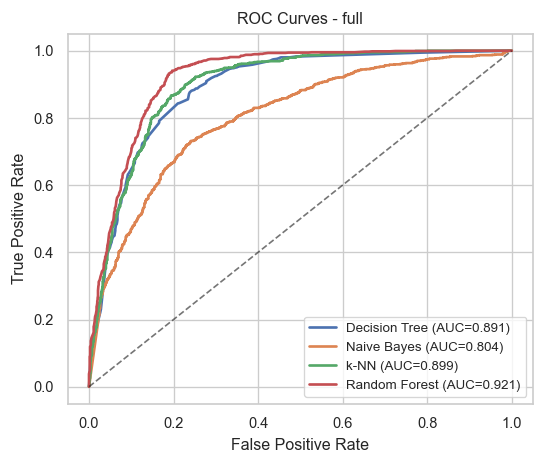
\includegraphics[width=0.9\linewidth]{roc_full.png}}
		\caption{ROC curves for the full-feature scenario. Random Forest dominates,
			followed by k-NN and the Decision Tree.}
		\label{fig:roc}
	\end{figure}

	\begin{figure}[htbp]
		\centerline{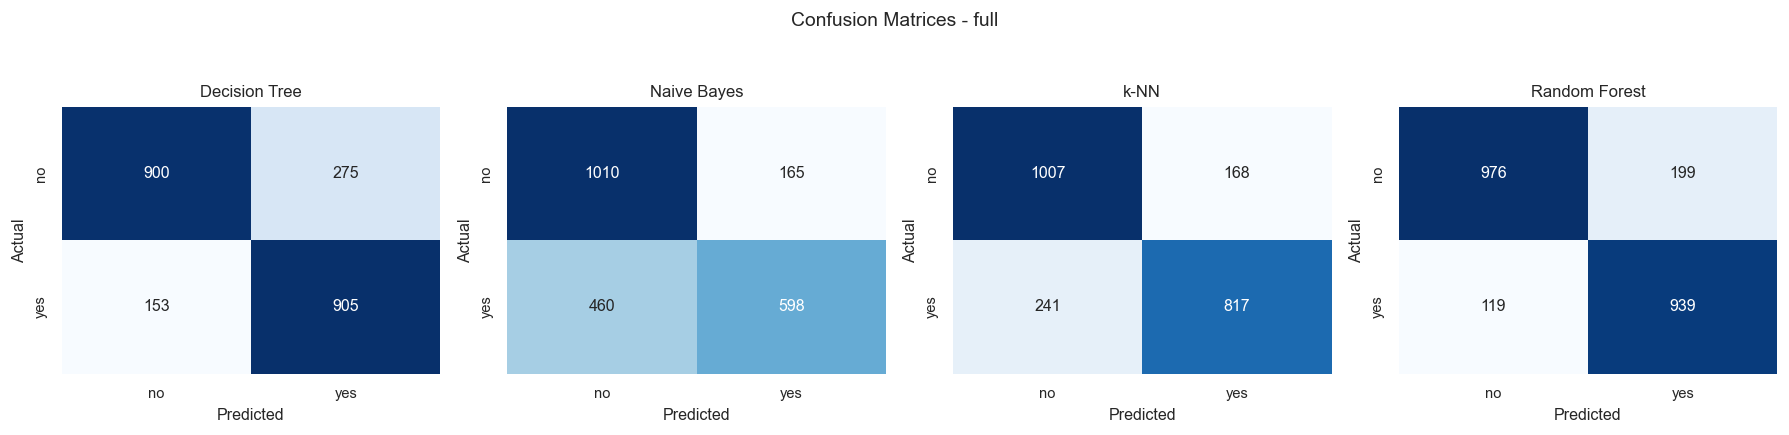
\includegraphics[width=\linewidth]{confusion_full.png}}
		\caption{Confusion matrices on the test set (full scenario). Random Forest
			achieves the most balanced error profile.}
		\label{fig:cm}
	\end{figure}

	\begin{figure}[htbp]
		\centerline{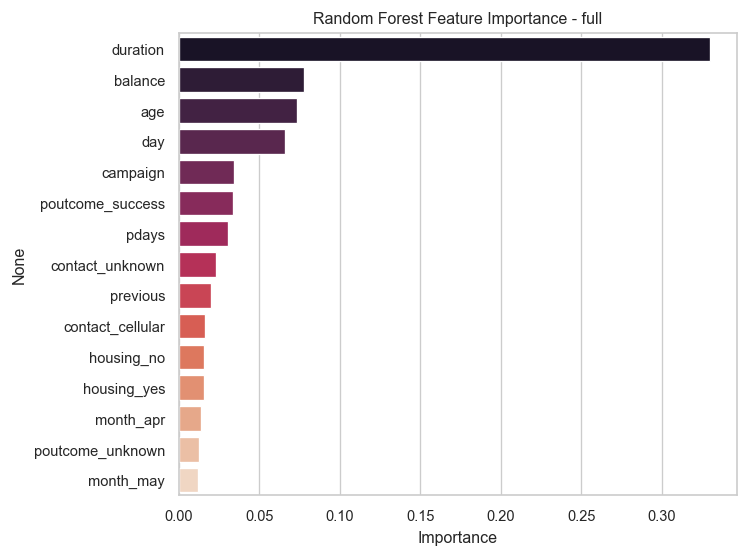
\includegraphics[width=0.82\linewidth]{feature_importance_full.png}}
		\caption{Random Forest feature importance (full scenario). Call duration is
			by far the most influential attribute.}
		\label{fig:fi}
	\end{figure}

	\begin{figure}[htbp]
		\centerline{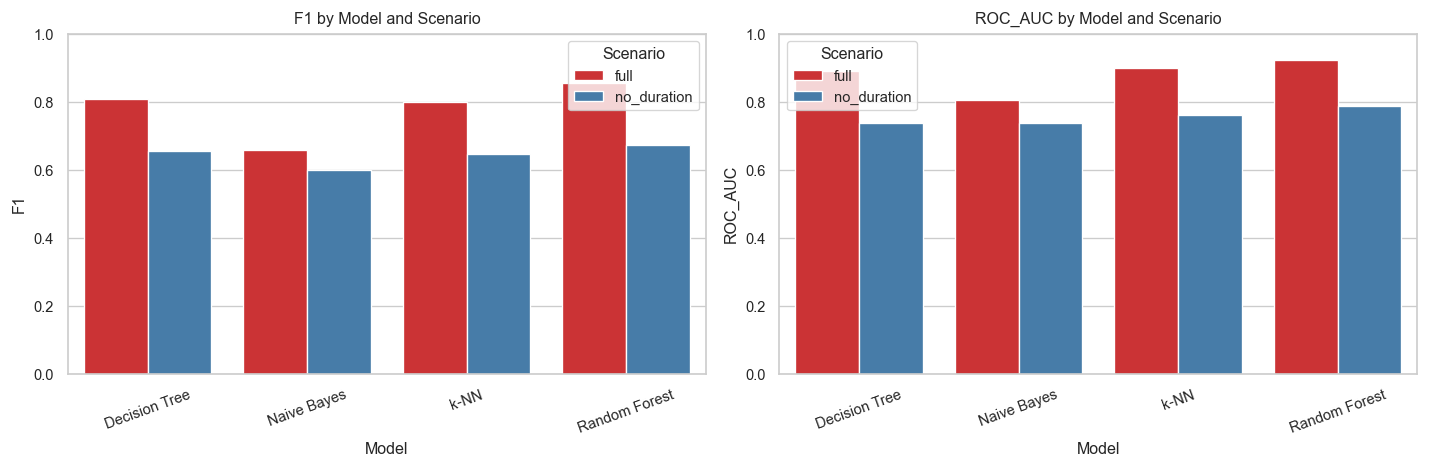
\includegraphics[width=\linewidth]{scenario_comparison.png}}
		\caption{F1 and ROC-AUC for each model in the two scenarios. Removing
			call duration lowers every model markedly.}
		\label{fig:scen}
	\end{figure}

	\subsection{Comparison of Approaches}
	Two conclusions follow from the comparison. First, across both scenarios
	Random Forest is the most accurate and highest-AUC model, confirming the
	expected advantage of ensembles over single learners; the improvement over the
	single Decision Tree (0.921 vs 0.891 AUC in the full scenario) is consistent
	with variance reduction from bagging. Second, the choice of input features
	matters far more than the choice of algorithm: moving from the full to the
	no-duration feature set costs Random Forest about 0.135 AUC, whereas the gap
	between the best and worst algorithm within a fixed scenario is smaller. This
	shows that data understanding, not just model selection, drives realistic
	performance.

	\section{Discussion}
	\label{sec:discussion}

	The best-performing method was Random Forest, and its advantage is explained by
	its ensemble nature: by averaging many de-correlated trees it captures
	non-linear interactions among mixed-type attributes while controlling the
	overfitting that a single deep tree would suffer. Naive Bayes performed worst
	because one-hot encoding produces many correlated binary features that violate
	its conditional-independence assumption.

	The most important finding concerns the \texttt{duration} attribute. It records
	the length of the last contact call, a value that is only known after the call
	has taken place and, as Fig.~\ref{fig:fi} shows, dominates the model. A long
	call typically means the client stayed engaged and is therefore close to
	subscribing, so \texttt{duration} is effectively a proxy for the outcome. Using
	it inflates performance (AUC 0.921) but produces a model that cannot be used
	for its intended purpose, namely deciding whom to call. When it is removed, the
	realistic ceiling drops to AUC 0.786. This is a textbook example of target
	leakage and matches the caution raised by the dataset's authors~\cite{b_moro}.

	The main \textbf{limitations} of this work are that it relies on a single,
	class-balanced snapshot of one bank's campaigns, so the absolute numbers may
	not transfer to other institutions or to the original imbalanced distribution;
	that only four classic algorithms were tried; and that hyperparameter grids
	were deliberately small to keep the study reproducible. A mildly
	\textbf{surprising} observation was how close k-NN came to Random Forest in the
	full scenario despite its simplicity, and how much the \texttt{poutcome}
	attribute, though 74.6\% unknown, still contributed useful signal for the
	minority of clients with a known prior outcome.

	Regarding data quality, the heavy use of the \texttt{unknown} token rather than
	true missing values meant that standard imputation was inappropriate; treating
	\texttt{unknown} as a category preserved its meaning and avoided introducing
	bias. Ethically, since attributes such as age, job, and marital status are
	predictive, a deployed model risks discriminating along these lines, and
	fairness auditing would be required before real use.

	\section{Conclusion and Future Work}
	\label{sec:conclusion}

	This project compared four classification algorithms for predicting bank
	term-deposit subscription on a balanced dataset of 11,162 client contacts.
	Random Forest was consistently the strongest model, reaching 0.858 accuracy and
	0.921 AUC with all features and remaining best (0.786 AUC) once the leaking
	call-duration attribute was removed. The central takeaway is that auditing
	features for leakage changed the conclusion about achievable performance far
	more than tuning or swapping algorithms did: the realistic, deployable model is
	the weaker-looking one.

	If more time were available, the study could be extended by (i) adding gradient
	boosting methods such as XGBoost and a simple neural network, (ii) repeating
	the experiment on the original imbalanced version of the dataset with
	resampling and cost-sensitive learning, (iii) applying model-agnostic
	explanations (e.g., SHAP) to interpret the no-duration model, and (iv)
	performing an explicit fairness analysis across demographic groups.

	\section*{AI Tool Use and Originality Declaration}
	\label{sec:ai_declaration}

	AI-assisted tools were used only for limited support, such as concept
	clarification, code debugging, code review, grammar improvement, and LaTeX
	formatting. The project idea, methodology choices, experiments, analysis,
	interpretation of results, and final report wording were reviewed, verified,
	and finalized by the student. The student accepts full responsibility for the
	accuracy, originality, reproducibility, and integrity of the submitted work.
	The disclosure levels below use the 0--6 scale defined in the project
	guidelines.

	\begin{table}[htbp]
		\caption{AI Use Disclosure Summary}
		\label{tab:ai_use}
		\centering
		\footnotesize
		\begin{tabular}{|p{0.35\linewidth}|c|p{0.38\linewidth}|}
			\hline
			\textbf{Project Stage} & \textbf{Level} & \textbf{Brief Description} \\
			\hline
			Conceptualization and idea generation & 2 & Topic and dataset options were briefly discussed with an AI tool; the research questions and final scope were decided by me. \\
			\hline
			Literature search and synthesis & 3 & Some candidate references were identified with AI support; I read and verified each source at first hand and wrote the synthesis in my own words. \\
			\hline
			Methodology, coding, and analysis & 2 & AI gave low-level support on a few coding and debugging steps; I assembled and ran the pipeline myself, verified every metric, and finalized the code. \\
			\hline
			Writing, editing, and LaTeX formatting & 4 & AI provided substantial help drafting and polishing the report text and LaTeX; I checked all reported numbers against my own outputs and finalized the wording. \\
			\hline
			Interpretation, discussion, and conclusion & 2 & Result interpretations were discussed at a high level with AI, but the analysis, discussion, and conclusions were written by me. \\
			\hline
		\end{tabular}
	\end{table}

	Do not list an AI tool as an author or as a source of factual claims.
	AI-generated references, explanations, code, figures, or numerical results were
	independently checked before inclusion.

	\begin{thebibliography}{00}

		\bibitem{b_moro} S.~Moro, P.~Cortez, and P.~Rita, ``A data-driven approach to
		predict the success of bank telemarketing,'' \textit{Decision Support
		Systems}, vol.~62, pp.~22--31, 2014.

		\bibitem{b_han} J.~Han, M.~Kamber, and J.~Pei, \textit{Data Mining: Concepts
		and Techniques}, 3rd~ed. Morgan Kaufmann, 2011.

		\bibitem{b_breiman} L.~Breiman, ``Random forests,'' \textit{Machine
		Learning}, vol.~45, no.~1, pp.~5--32, 2001.

		\bibitem{b_quinlan} J.~R.~Quinlan, ``Induction of decision trees,''
		\textit{Machine Learning}, vol.~1, no.~1, pp.~81--106, 1986.

		\bibitem{b_sklearn} F.~Pedregosa et al., ``Scikit-learn: Machine learning in
		Python,'' \textit{Journal of Machine Learning Research}, vol.~12,
		pp.~2825--2830, 2011.

	\end{thebibliography}

	\newpage
	\appendix

	\section{Code Repository}
	\label{app:code}

	Full source code is available at:
	\url{https://github.com/dorukdolas/BIL-476-Project}

	The repository contains \texttt{src/config.py} (paths and constants),
	\texttt{src/eda.py} (exploratory analysis and figures), and
	\texttt{src/experiments.py} (preprocessing, model training, evaluation, and all
	result figures/tables), together with \texttt{requirements.txt} and a
	\texttt{README}. Listing~\ref{lst:core} shows the core modeling loop.

	\begin{lstlisting}[caption={Core preprocessing and model-selection loop}, label={lst:core}]
pre = ColumnTransformer([
    ("num", StandardScaler(), numeric_features),
    ("cat", OneHotEncoder(handle_unknown="ignore"),
     categorical_features),
])
cv = StratifiedKFold(n_splits=5, shuffle=True,
                     random_state=42)
for name, (estimator, grid) in model_grid().items():
    pipe = Pipeline([("pre", pre), ("clf", estimator)])
    search = GridSearchCV(pipe, grid, scoring="roc_auc",
                          cv=cv, n_jobs=-1)
    search.fit(X_train, y_train)
    best = search.best_estimator_
    y_proba = best.predict_proba(X_test)[:, 1]
	\end{lstlisting}

	\section{Additional Figures}
	\label{app:additional}

	Fig.~\ref{fig:num} shows the numeric attribute distributions by class, and
	Fig.~\ref{fig:corr} shows the correlation matrix of the numeric attributes,
	which is weak overall and justifies keeping all numeric features.

	\begin{figure}[htbp]
		\centerline{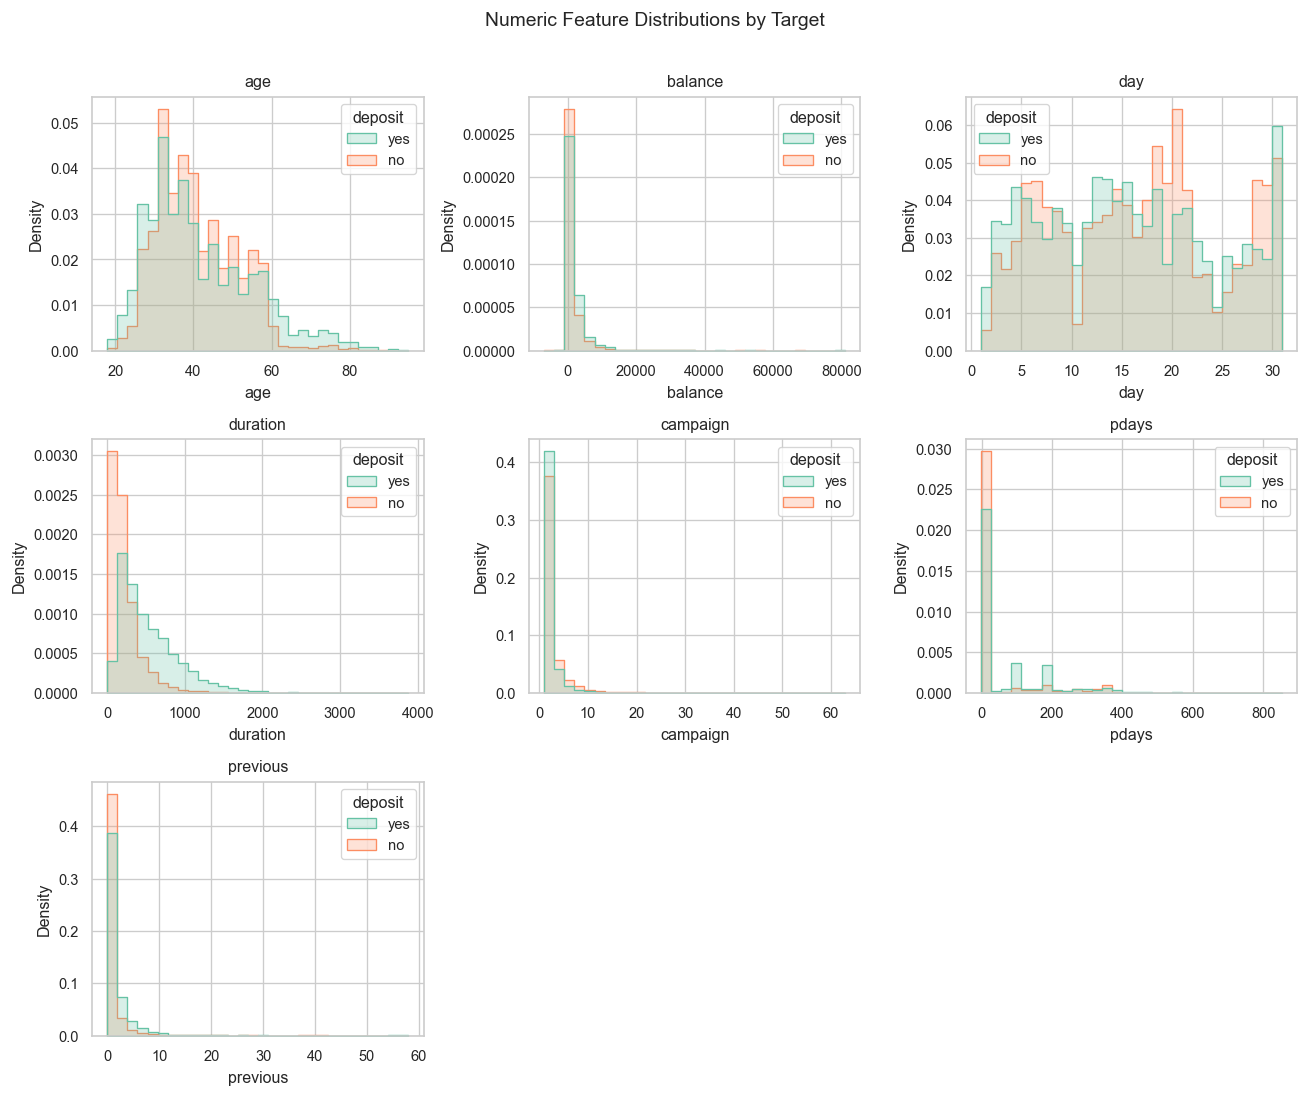
\includegraphics[width=\linewidth]{numeric_distributions.png}}
		\caption{Numeric attribute distributions by target class.}
		\label{fig:num}
	\end{figure}

	\begin{figure}[htbp]
		\centerline{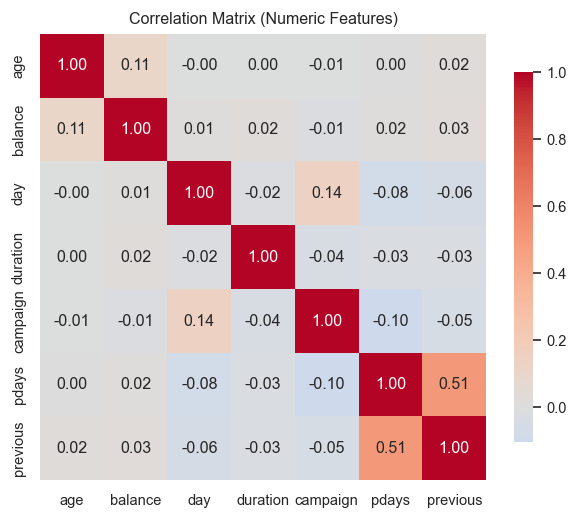
\includegraphics[width=0.8\linewidth]{correlation_matrix.png}}
		\caption{Correlation matrix of numeric attributes. Correlations are weak,
			indicating little redundancy among numeric features.}
		\label{fig:corr}
	\end{figure}

\end{document}
